Для распространения и установки программного комплекса <<COEX>> на электронные вычислительные машины был выбран формат двоичного пакета *.deb. Данный пакет включает в себя все необходимые файлы для работы программы, а также содержит список зависимостей. Он имеет строго типизированную структуру и используется операционными системами Unix. Строго типизированная структура позволяет операционной системе узнавать все нужные элементы для установки и работы с данным пакетам вне зависимости от программного обеспечения (далее ПО), находящейся в данном Deb-пакете, узнавать зависимости программных библиотек, необходимых для запуска программного продукта, содержащегося в двоичном пакете.  Выбор данного формата пакета обусловлен возможностью его гибкой настройки для любого программного обеспечения (возможность использовать встроенные скрипты для настройки процесса установки ПО), поддержкой почти всеми операционными системами Unix. А также широкой распространенностью использования deb-пакетов в семействе операционных систем Unix в связи с высокой популярностью дистрибутивов операционных систем, в которой он распространяется.~\cite{tecmint}  

Для пакета *.deb содержащего программный комплекс <<COEX>> ранее использовалась ссылка на репозиторий содержащий данный пакет для его дальнейшей установки. При появление новой версии программного комплекса <<COEX>> создается новый deb пакет, после чего пользователю нужно было зайти на сайт программного комплекса <<COEX>>, и скачать новый deb пакет данного комплекса. Для автоматизации данного процесса было написаны две программы, а также настроена операционная утилита cron для запуска программ в определенный промежуток времени, определяемый в конфигурационном файле cron. Первая программа запрашивает у пользователя права на внесение изменений в конфигурационный файл sources.list, затем находит данный файл и вносит изменения (рисунок~\ref{ser_1:ser_1}). 

\begin{figure}[h!]
\center{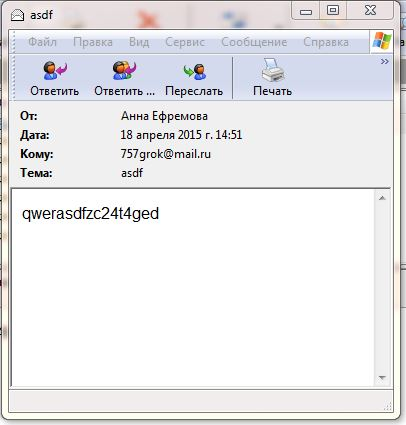
\includegraphics[width=0.7\linewidth]{ser_1}}
\caption{ Программа для внесения изменений в sources.list }
\label{ser_1:ser_1}
\end{figure}

Изменения включают в себя адрес до репозитория   в сети Internet, где хранится deb пакет программного комплекса <<COEX>>, а также запись ключа, которым подписывают скаченные файлы с репозитория, вносятся также команды по установки и обновлению пакета при скачивании через менеджера. Данные действия позволяет менеджеру обновлений операционной системы Linux следить за версиями deb пакета в репозиторие, содержащего программный комплекс <<COEX>>, при появление новой версии менеджер сообщит пользователю о возможном обновлении. Первая программа находится на сайте проекта <<COEX>>, скачивается и запускается пользователем. 

Вторая программа находится на сервере с репозиториям, и с помощью системной утилиты CRON запускается в определенное время, при наличии изменений из ветки master в системе контроля версий git (рисунок~\ref{ser_2:ser_2}).

\begin{figure}[h!]
\center{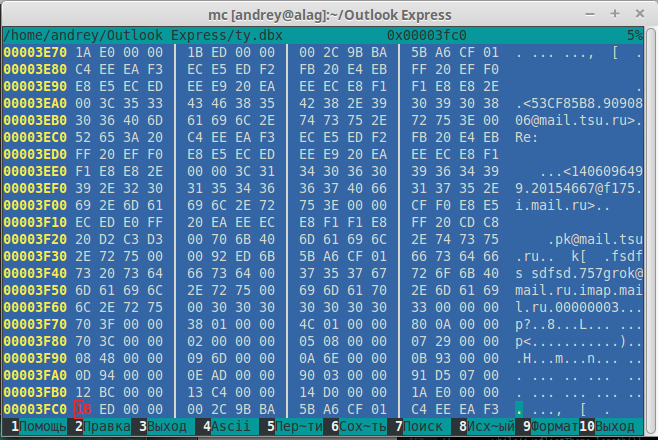
\includegraphics[width=0.7\linewidth]{ser_2}}
\caption{ Программа  для запуска сборки по времени  с помощью демона  «CRON» }
\label{ser_2:ser_2}
\end{figure}

Скрипт-программа на основе сведений из системы контроля версий GIT проекта <<COEX>>, создает версию для двоичного пакета формата deb, сам deb пакет создается при помощи скрипт-программы по созданию  deb пакета из тексты программ проекта (рисунок~\ref{ser_3:ser_3}).

\begin{figure}[h!]
\center{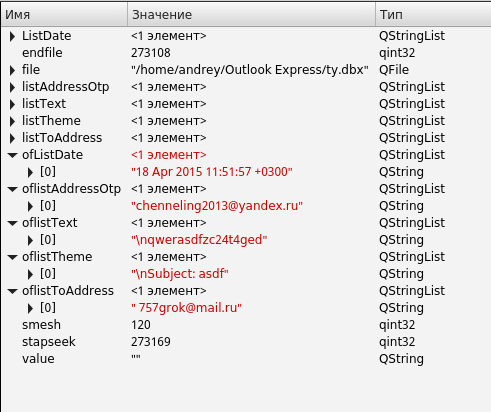
\includegraphics[width=0.7\linewidth]{ser_3}}
\caption{ Программа для присвоения версии }
\label{ser_3:ser_3}
\end{figure}

Тестирование проводилось, на операционной системе «Debian 8.4», и ее наследниках(Ubuntu(16.04), Mint (17.3))(рисунки~\ref{ser_4:ser_4}-~\ref{ser_6:ser_6}).

\begin{figure}[h!]
\center{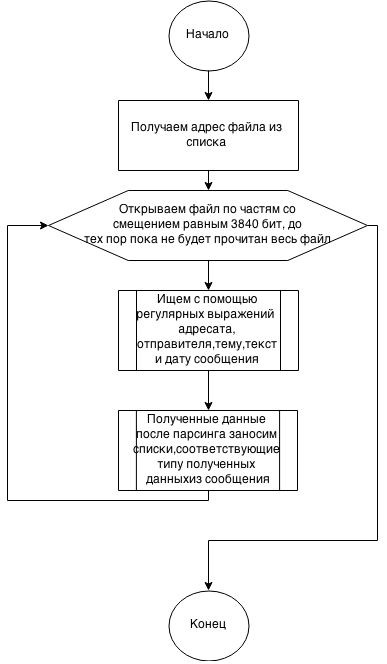
\includegraphics[width=0.7\linewidth]{ser_4}}
\caption{ Установка на Debian }
\label{ser_4:ser_4}
\end{figure}

\begin{figure}[h!]
\center{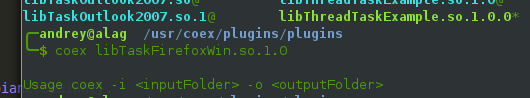
\includegraphics[width=0.7\linewidth]{ser_5}}
\caption{ Установка на Mint }
\label{ser_5:ser_5}
\end{figure}

\begin{figure}[h!]
\center{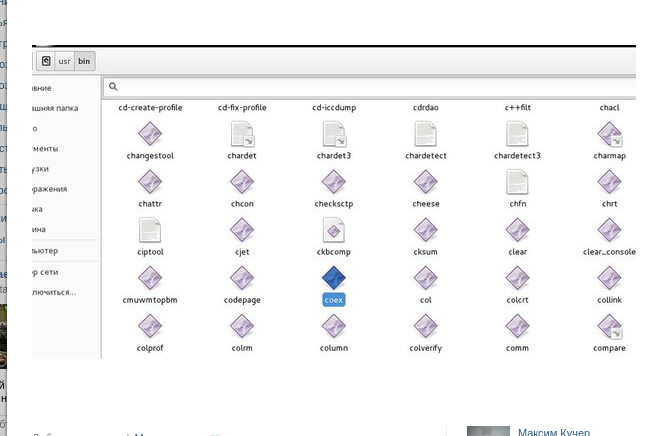
\includegraphics[width=0.7\linewidth]{ser_6}}
\caption{ Установка на Ubuntu }
\label{ser_6:ser_6}
\end{figure}

В ходе тестирования проверялось корректность работы двоичного пакета после прохождения автоматизированной сборки, также проверялась функционирование программного комплекса <<COEX>>, и корректность удаления проекта с компьютера пользователя. Результатом тестирования были выявлены проблемы с некаторами зависимостями модулей, и связи модулей c программным ядром <<COEX>>. После выявления проблем были перепроверены и исправлены зависимости, в модулях где были найдены ошибки с зависимостями. А также переделана структура пакета, для исправления проблемы взаимодействия ядра <<COEX>> и его модулей при установке через двоичный пакет.  

\clearpage
